\documentclass[conference]{IEEEtran}

\usepackage[pdftex]{graphicx}
% \usepackage{amsmath}
% \usepackage{afterpage}
% \usepackage{wrapfig}
% \usepackage{tabularx}
% \usepackage{subfigure}
\usepackage{caption}
\usepackage{xcolor}
% \usepackage{tabu}
% \usepackage{booktabs}
% \usepackage{multicol}
% \usepackage{hyperref}

\hyphenation{op-tical net-works semi-conduc-tor}

% \usepackage[switch]{lineno}
% \linenumbers
% \modulolinenumbers[10]

\begin{document}

\title{DQM4HEP : A generic\\Data Quality Monitoring for High Energy Physics}

\author{

\IEEEauthorblockN{R\'emi \'Et\'e}
\IEEEauthorblockA{Univ, Lyon, Universit\'e Lyon 1, \\
CNRS/IN2P3, IPNL 4 rue E Fermi \\
69622, Villeurbanne CEDEX, France\\
Email: rete@ipnl.in2p3.fr}

\and

\IEEEauthorblockN{Antoine Pingault}
\IEEEauthorblockA{Ghent University, Department of Physics \\
and Astronomy Proeftuinstraat 86,\\
B-9000 Gent, Belgium\\
Email: antoine.pingault@ugent.be}

\and

\IEEEauthorblockN{Laurent Mirabito}
\IEEEauthorblockA{Univ, Lyon, Universit\'e Lyon 1, \\
CNRS/IN2P3, IPNL 4 rue E Fermi \\
69622, Villeurbanne CEDEX, France\\
Email: mirabito@ipnl.in2p3.fr}

}

\maketitle

\IEEEpeerreviewmaketitle

\section{Introduction}

With increasingly sophisticated experiment, online Data Quality Monitoring (DQM) is of a significant importance for the detector and operation efficiency. Monitoring data is also a first step to the certification of the recorded data for off-line physics analysis. Usually, monitoring systems are developed and built on top of the Event Data Model (EDM) and leads to a strong dependency to the data format and storage. In order to increase the flexibility and porting of software across experiments, a generic online Data Quality Monitoring system has been developed without any assumption on the Event Data Model and data type to treat.

In addition, a dedicated implementation, based on the LCIO~\cite{LCIO} Event Data Model for the Linear Collider Collaboration, was also developed. This implementation will be put to real condition testing using a combined detector setup with the CALICE~\footnote{CAlorimeter for LInear Collider Experiment} Semi-Digital Hadronic CALorimeter (SDHCAL) and Silicon Tungsten Electronic Calorimeter (SiWECal) prototypes during coming test beam campaigns at CERN\footnote{Conseil Européen pour la Recherche Nucléaire}.

\section{Key points and software architecture}

The framework is based on a plugin system. The data serialization used to send data across the network is encapsulated in plugins loaded at run-time. It is designed to be run in separate processes linked to each other by TCP/IP or HTTP protocols using DIM\cite{DIM} and Mongoose\cite{MONGOOSE} respectively.

\begin{figure}[htbp]
  \begin{center}
    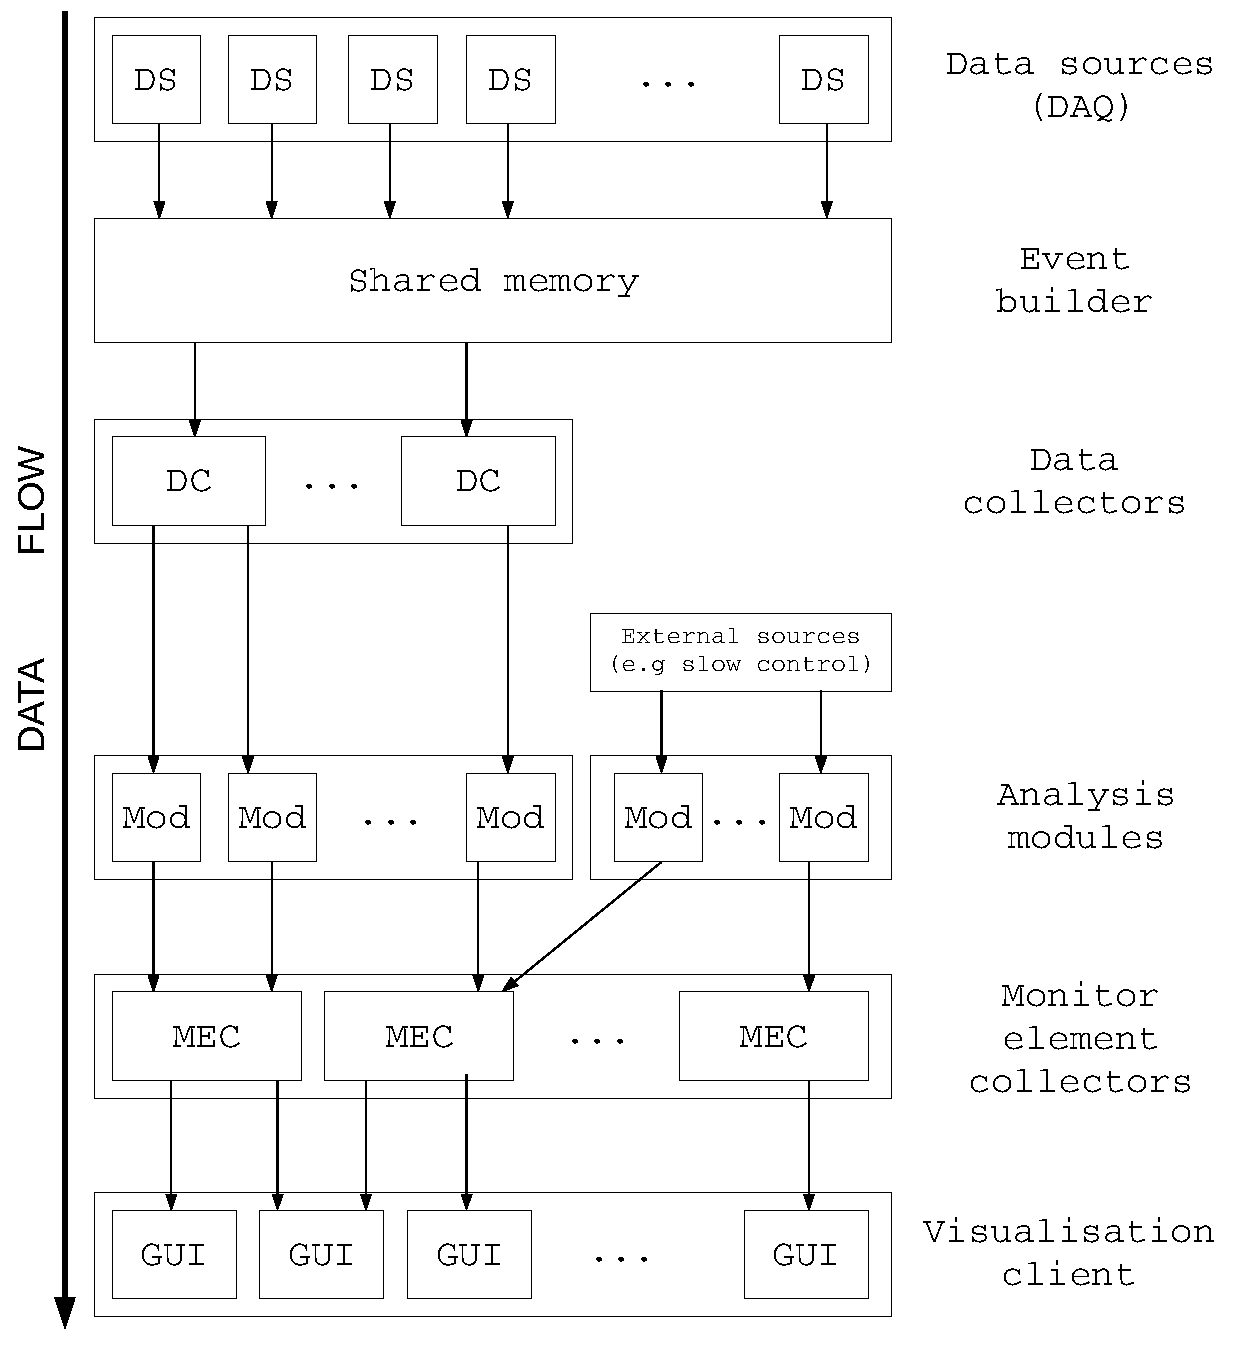
\includegraphics[width=0.8\linewidth]{DQMWorkflow.pdf}
    \caption{\label{DQM_WORKFLOW}The monitoring framework data flow: from data sources to visualization.}
  \end{center}
  \vspace{-.95cm}
\end{figure}


Fig.~\ref{DQM_WORKFLOW} shows the monitoring framework data flow from incoming data sources to the client visualization machines. A significant effort has been put on the creation of a generic interface to the data acquisition system and the development of an event builder. An independent data acquisition (DAQ) process dumps the content of data sources within the shared memory (\textit{shm}) until a given limit in bytes is reached (set by the DAQ). In this way, a slower data treatment by the monitoring will not affect the data taking and writing to disk. Since the data structure depends on the setup of the experiment, the implementation of the event builder becomes highly specific. The event building is encapsulated in series of \textit{shm processors} which convert data sources buffers into the user data structure. The whole reconstructed event is then serialized, dispatched across the network and stored into one or multiple data collector server applications.
A client interface is provided to perform queries on collected data, either manually or in an automated way. This automatic mode, referred to as update mode later, republish data to registered client as soon as they are available.
User's online data analysis are also implemented as plugins in the system and steered using configuration files, increasing the modularity of the framework. They use a data collector client interface in update mode to receive and process data.

The original goal of the online data analysis is to reduce the initial amount of data to a few monitorable quantities summarizing its quality and the status of the detection systems. Such quantities have been encapsulated in a unique interface called \textit{monitor element}. To evaluate the data quality, built-in template tests are provided and are frequently processed by the system. A user API is provided for the online analysis module to book \textit{monitor elements} and their quality tests which are then published across the network. They are in their turn collected by server applications and distributed to visualization clients, again, either thanks to manual queries or in update mode.

To visualize \textit{monitor elements} from the collectors, a Graphical User Interface (GUI) has been developed using the Qt\cite{QT} toolkit. It can use multiple client interfaces to every available collectors on the network. The user can then display received \textit{monitor elements} in areas organized in tabs. Multiple configurations with different sets of \textit{monitor elements} can be set-up at once. This allows for a quick overview of all the critical elements and variables needed for the good operation of the experiment.


%%%%%%%%%%%%%%%%%%%%%%%%%%%%%%%%%%%%%%%%%%%%%%%%%%%%%%%%%%%%%%%%%%%
%%%%%%%%%%%%%%%%%%%%%%%%%%%%%%%%%%%%%%%%%%%%%%%%%%%%%%%%%%%%%%%%%%%
\section{Implementation and tests}
In order to test the framework, a dedicated implementation has been developed for the CALICE collaboration and its SDHCAL and SiWEcal prototypes.
An interface to read and write events in the LCIO format has been written using our generic data streaming toolkit named \textit{xdrstream}.

%%%%%%%%%%%%%%%%%%%%%%%%%%%%%%%%%%%%%%%%%%%%%%%%%%%%%%%%%%%%%%%%%%%

As mentioned previously, the CALICE-SDHCAL collaboration developed tools to dump online raw data coming from the detectors to a shared memory space as data source buffers. To treat these buffers, we implemented a dedicated \textit{shm processor} plugin. It reads the data sent by the DAQ system into the shared memory, then call the online event builder (\textit{levbdim}) to reconstruct data into the LCIO format. The reconstructed event is eventually sent over the network to the event collector.

The LCIO EDM contains multiple data structures for different levels of reconstruction that analysis can use. Data converters are provided to pass from one LCIO data structure to the other. This gives the ability to plug off-line analysis into the monitoring system, leading to a better assessment of the overall data quality.

The monitoring system can also be tested with LCIO data files as a data source. In order to keep conditions as close as possible to a real setup, it can be configured to simulate the timing structure of the raw data.

%%%%%%%%%%%%%%%%%%%%%%%%%%%%%%%%%%%%%%%%%%%%%%%%%%%%%%%%%%%%%%%%%%%
For the test beam campaign at CERN, specific analysis aimed to the monitoring of the SDHCAL and SiWEcal have also been developed. They come as independent modules to plug into the framework and can be started or stopped at any given time. All the modules are configurable either through xml files or command line: most of the parameters can be quickly adjusted a few seconds prior to start the module.

Part of our implementation includes a module to watch the slow control parameters (high and low voltages, pressure, temperature, etc.). It is developed as a standalone module since the source of these data is not a data collector but an external source as shown in Fig.~\ref{DQM_WORKFLOW}.

One analysis is dedicated to the raw data study and permits the shifters to quickly discover and try to correct for noisy part of the detector. A beam study analysis is available to display metrics about the beam spill such as its length, time structure, number of acquisition cycle per spill, etc. Some \textit{monitor elements} from this module can also be used as performances indicators for the framework. One practical example would be the ratio between the number of events treated by the monitoring and the DAQ systems.

Other modules are dedicated to efficiency measurement of some parts of the detectors, particle identification or tracking. Specific information using core properties of the detectors are also recorded, like the deposited energy (SiWEcal) or number of hits for each threshold (SDHCAL). Finally, event display modules are also present to visualise particle interactions inside the detectors.

The Marlin\cite{MARLIN} framework being widely used within the Linear Collider Collaboration for data analysis, an interface is under development and will permit users to directly plug their analysis as it is into the monitoring.

The framework has been successfully tested with off-line SDHCAL data from previous tests beam using the time structure of the beam spills. Successful online tests were also performed by taking cosmic muons data with the same deployment scheme foreseen for the full scale testing at CERN. For this campaign, the framework will be deployed across multiple computers, each one running a set of collectors (\textit{monitor element} and event) and analysis modules. Several monitoring GUIs will be running on these computers and personal shifters equipment.


\section{Conclusion}
In light of the critical importance of a tool to quickly detect problems and ensure a good data quality, a new generic framework for Data Quality Monitoring systems has been created, integrating full flexibility across experiment setup.

Contrary to most systems available for High Energy Physics up to now, it is not tied to a given experiment set-up. All the tools needed to develop a specific implementation depending on specificities of the experiment, such as DAQ interface, data format and detector analysis, are provided within the framework.

To put to test this system, a dedicated implementation has been developed in parallel for the CALICE SDHCAL and SiWEcal collaborations.
The whole system has been successfully tested with the CALICE SDHCAL prototype with offline data and online cosmic muons.  It will be put to full scale testing during a two weeks test beam campaign at CERN with the CALICE SDHCAL and SiWEcal prototypes. The framework being in its final stage and given successful SDHCAL tests, satisfactory results are expected.

\begin{thebibliography}{1}

\bibitem{LCIO}
% Frank Gaede, \emph{\tt lcio.desy.de}, 2016.
S. Aplin et al., "LCIO: A persistency framework and event data model for HEP", \emph{Nuclear Science Symp. and Medical Imaging Conf. (NSS/MIC), 2012 IEEE}, Anaheim, CA, 2012, pp. 2075-2079.

\bibitem{DIM}
C. Gaspar et al., "DIM, a Portable, Light Weight Package for Information Publishing, Data Transfer and Inter-process Communication" presented at the \emph{Int. Conf. Computing in High Energy and Nuclear Physics}, Padova, Italy, 2000)

\bibitem{MONGOOSE}
Michael J Hammel, "Mongoose: an embeddable web server in C", \emph{Linux Journal}, 2010, pp. 192

\bibitem{QT}
% J. Blanchette and M. Summerfield
Qt Company, \emph{\tt http://www.qt.io}, v4.7, 2016.

\bibitem{ROOT}
Rene Brun and Fons Rademakers, "ROOT - An Object Oriented Data Analysis Framework", \emph{Nucl. Inst. \& Meth. in Phys. Res. A 389}, 1997, pp. 81-86. Available: http://root.cern.ch/

\bibitem{MARLIN}
F. Gaede,  "Marlin and LCCD: Software tools for the ILC", \emph{Nucl. Inst. \& Meth. A559}, 2006, pp. 177-180

\end{thebibliography}

\end{document}
